% % % % mainfile: ../../../../master.tex
\label{task:20240515_android}

\subsection{Verify debloater in several android apps}

\begin{lstlisting}
05-15 21:44:13.512     0     0 E SELinux : avc:  denied  { find } for pid=2247 uid=99007 name=content_capture scontext=u:r:isolated_app:s0:c512,c768 tcontext=u:object_r:content_capture_service:s0 tclass=service_manager permissive=0
05-15 21:44:13.493  2247  2247 F ocessService1:0: thread.cc:2517] No pending exception expected: java.lang.SecurityException: Isolated process not allowed to call getContentProvider
05-15 21:44:13.493  2247  2247 F ocessService1:0: thread.cc:2517]   at java.lang.Exception android.os.Parcel.createExceptionOrNull(int, java.lang.String) (Parcel.java:3057)
05-15 21:44:13.493  2247  2247 F ocessService1:0: thread.cc:2517]   at java.lang.Exception android.os.Parcel.createException(int, java.lang.String) (Parcel.java:3041)
05-15 21:44:13.493  2247  2247 F ocessService1:0: thread.cc:2517]   at void android.os.Parcel.readException(int, java.lang.String) (Parcel.java:3024)
05-15 21:44:13.493  2247  2247 F ocessService1:0: thread.cc:2517]   at void android.os.Parcel.readException() (Parcel.java:2966)
05-15 21:44:13.493  2247  2247 F ocessService1:0: thread.cc:2517]   at android.app.ContentProviderHolder android.app.IActivityManager$Stub$Proxy.getContentProvider(android.app.IApplicationThread, java.lang.String, java.lang.String, int, boolean) (IActivityManager.java:5935)
05-15 21:44:13.493  2247  2247 F ocessService1:0: thread.cc:2517]   at android.content.IContentProvider android.app.ActivityThread.acquireProvider(android.content.Context, java.lang.String, int, boolean) (ActivityThread.java:7381)
05-15 21:44:13.493  2247  2247 F ocessService1:0: thread.cc:2517]   at android.content.IContentProvider android.app.ContextImpl$ApplicationContentResolver.acquireUnstableProvider(android.content.Context, java.lang.String) (ContextImpl.java:3668)
05-15 21:44:13.493  2247  2247 F ocessService1:0: thread.cc:2517]   at android.content.IContentProvider android.content.ContentResolver.acquireUnstableProvider(android.net.Uri) (ContentResolver.java:2542)
05-15 21:44:13.493  2247  2247 F ocessService1:0: thread.cc:2517]   at android.database.Cursor android.content.ContentResolver.query(android.net.Uri, java.lang.String[], android.os.Bundle, android.os.CancellationSignal) (ContentResolver.java:1213)
05-15 21:44:13.493  2247  2247 F ocessService1:0: thread.cc:2517]   at android.database.Cursor android.content.ContentResolver.query(android.net.Uri, java.lang.String[], java.lang.String, java.lang.String[], java.lang.String, android.os.CancellationSignal) (ContentResolver.java:1161)
05-15 21:44:13.493  2247  2247 F ocessService1:0: thread.cc:2517]   at android.database.Cursor android.content.ContentResolver.query(android.net.Uri, java.lang.String[], java.lang.String, java.lang.String[], java.lang.String) (ContentResolver.java:1117)
05-15 21:44:13.493  2247  2247 F ocessService1:0: thread.cc:2517]   at java.lang.Class java.lang.VMClassLoader.findLoadedClass(java.lang.ClassLoader, java.lang.String) (VMClassLoader.java:-2)
05-15 21:44:13.493  2247  2247 F ocessService1:0: thread.cc:2517]   at java.lang.Class java.lang.ClassLoader.findLoadedClass(java.lang.String) (ClassLoader.java:738)
05-15 21:44:13.493  2247  2247 F ocessService1:0: thread.cc:2517]   at java.lang.Class java.lang.ClassLoader.loadClass(java.lang.String, boolean) (ClassLoader.java:363)
05-15 21:44:13.493  2247  2247 F ocessService1:0: thread.cc:2517]   at java.lang.Class java.lang.ClassLoader.loadClass(java.lang.String) (ClassLoader.java:312)
05-15 21:44:13.493  2247  2247 F ocessService1:0: thread.cc:2517]   at android.app.Service android.app.AppComponentFactory.instantiateService(java.lang.ClassLoader, java.lang.String, android.content.Intent) (AppComponentFactory.java:129)
05-15 21:44:13.493  2247  2247 F ocessService1:0: thread.cc:2517]   at void android.app.ActivityThread.handleCreateService(android.app.ActivityThread$CreateServiceData) (ActivityThread.java:4667)
05-15 21:44:13.493  2247  2247 F ocessService1:0: thread.cc:2517]   at void android.app.ActivityThread.-$$Nest$mhandleCreateService(android.app.ActivityThread, android.app.ActivityThread$CreateServiceData) (ActivityThread.java:-1)
05-15 21:44:13.493  2247  2247 F ocessService1:0: thread.cc:2517]   at void android.app.ActivityThread$H.handleMessage(android.os.Message) (ActivityThread.java:2289)
05-15 21:44:13.493  2247  2247 F ocessService1:0: thread.cc:2517]   at void android.os.Handler.dispatchMessage(android.os.Message) (Handler.java:106)
05-15 21:44:13.493  2247  2247 F ocessService1:0: thread.cc:2517]   at boolean android.os.Looper.loopOnce(android.os.Looper, long, int) (Looper.java:205)
05-15 21:44:13.493  2247  2247 F ocessService1:0: thread.cc:2517]   at void android.os.Looper.loop() (Looper.java:294)
05-15 21:44:13.493  2247  2247 F ocessService1:0: thread.cc:2517]   at void android.app.ActivityThread.main(java.lang.String[]) (ActivityThread.java:8248)
05-15 21:44:13.493  2247  2247 F ocessService1:0: thread.cc:2517]   at java.lang.Object java.lang.reflect.Method.invoke(java.lang.Object, java.lang.Object[]) (Method.java:-2)
05-15 21:44:13.493  2247  2247 F ocessService1:0: thread.cc:2517]   at void com.android.internal.os.RuntimeInit$MethodAndArgsCaller.run() (RuntimeInit.java:552)
05-15 21:44:13.493  2247  2247 F ocessService1:0: thread.cc:2517]   at void com.android.internal.os.ChildZygoteInit.runZygoteServer(com.android.internal.os.ZygoteServer, java.lang.String[]) (ChildZygoteInit.java:136)
05-15 21:44:13.493  2247  2247 F ocessService1:0: thread.cc:2517]   at void com.android.internal.os.WebViewZygoteInit.main(java.lang.String[]) (WebViewZygoteInit.java:147)
05-15 21:44:13.493  2247  2247 F ocessService1:0: thread.cc:2517]   at java.lang.Object java.lang.reflect.Method.invoke(java.lang.Object, java.lang.Object[]) (Method.java:-2)
05-15 21:44:13.493  2247  2247 F ocessService1:0: thread.cc:2517]   at void com.android.internal.os.RuntimeInit$MethodAndArgsCaller.run() (RuntimeInit.java:552)
05-15 21:44:13.493  2247  2247 F ocessService1:0: thread.cc:2517]   at void com.android.internal.os.ZygoteInit.main(java.lang.String[]) (ZygoteInit.java:971)
05-15 21:44:13.493  2247  2247 F ocessService1:0: thread.cc:2517] Caused by: android.os.RemoteException: Remote stack trace:
05-15 21:44:13.493  2247  2247 F ocessService1:0: thread.cc:2517] 	at com.android.server.am.ActivityManagerService.enforceNotIsolatedCaller(ActivityManagerService.java:3079)
05-15 21:44:13.493  2247  2247 F ocessService1:0: thread.cc:2517] 	at com.android.server.am.ContentProviderHelper.getContentProvider(ContentProviderHelper.java:130)
05-15 21:44:13.493  2247  2247 F ocessService1:0: thread.cc:2517] 	at com.android.server.am.ActivityManagerService.getContentProvider(ActivityManagerService.java:6782)
05-15 21:44:13.493  2247  2247 F ocessService1:0: thread.cc:2517] 	at android.app.IActivityManager$Stub.onTransact(IActivityManager.java:2776)
05-15 21:44:13.493  2247  2247 F ocessService1:0: thread.cc:2517] 	at com.android.server.am.ActivityManagerService.onTransact(ActivityManagerService.java:2763)
05-15 21:44:13.493  2247  2247 F ocessService1:0: thread.cc:2517] 
05-15 21:44:13.493  2247  2247 F ocessService1:0: thread.cc:2517] (Throwable with no stack trace)
\end{lstlisting}

In AOSP 13, the runtime responses to the changes in the schema by the Management App instantly, whereas in AOSOP 14, the response is not consistent. Now trying to go into \path{MY_match_target_method} of \path{art/runtime/runtime.cc} and see the flow up close.

The debloating works perfectly when:
\begin{lstlisting}
adb uninstall com.atomic.apps.medical.drug.dictionary && adb install success_apps/60_com.atomic.apps.medical.drug.dictionary.apk 
\end{lstlisting}
But after closing the app and relaunch, the debloating doesn't work for some methods anymore. Need to see what happens to the runtime when the app is closed and relaunched.

This sandbox related exception has nothing to do with this error as it still shows when the debloating was working perfectly after reinstalling:
\begin{lstlisting}
05-16 01:06:34.222  2319  2319 F ocessService1:0: thread.cc:2517] No pending exception expected: java.lang.SecurityException: Isolated process not allowed to call getContentProvider
05-16 01:06:34.222  2319  2319 F ocessService1:0: thread.cc:2517]   at java.lang.Exception android.os.Parcel.createExceptionOrNull(int, java.lang.String) (Parcel.java:3057)
05-16 01:06:34.222  2319  2319 F ocessService1:0: thread.cc:2517]   at java.lang.Exception android.os.Parcel.createException(int, java.lang.String) (Parcel.java:3041)
05-16 01:06:34.222  2319  2319 F ocessService1:0: thread.cc:2517]   at void android.os.Parcel.readException(int, java.lang.String) (Parcel.java:3024)
05-16 01:06:34.222  2319  2319 F ocessService1:0: thread.cc:2517]   at void android.os.Parcel.readException() (Parcel.java:2966)
05-16 01:06:34.222  2319  2319 F ocessService1:0: thread.cc:2517]   at android.app.ContentProviderHolder android.app.IActivityManager$Stub$Proxy.getContentProvider(android.app.IApplicationThread, java.lang.String, java.lang.String, int, boolean) (IActivityManager.java:5935)
05-16 01:06:34.222  2319  2319 F ocessService1:0: thread.cc:2517]   at android.content.IContentProvider android.app.ActivityThread.acquireProvider(android.content.Context, java.lang.String, int, boolean) (ActivityThread.java:7381)
05-16 01:06:34.222  2319  2319 F ocessService1:0: thread.cc:2517]   at android.content.IContentProvider android.app.ContextImpl$ApplicationContentResolver.acquireUnstableProvider(android.content.Context, java.lang.String) (ContextImpl.java:3668)
05-16 01:06:34.222  2319  2319 F ocessService1:0: thread.cc:2517]   at android.content.IContentProvider android.content.ContentResolver.acquireUnstableProvider(android.net.Uri) (ContentResolver.java:2542)
05-16 01:06:34.222  2319  2319 F ocessService1:0: thread.cc:2517]   at android.database.Cursor android.content.ContentResolver.query(android.net.Uri, java.lang.String[], android.os.Bundle, android.os.CancellationSignal) (ContentResolver.java:1213)
05-16 01:06:34.222  2319  2319 F ocessService1:0: thread.cc:2517]   at android.database.Cursor android.content.ContentResolver.query(android.net.Uri, java.lang.String[], java.lang.String, java.lang.String[], java.lang.String, android.os.CancellationSignal) (ContentResolver.java:1161)
05-16 01:06:34.222  2319  2319 F ocessService1:0: thread.cc:2517]   at android.database.Cursor android.content.ContentResolver.query(android.net.Uri, java.lang.String[], java.lang.String, java.lang.String[], java.lang.String) (ContentResolver.java:1117)
05-16 01:06:34.222  2319  2319 F ocessService1:0: thread.cc:2517]   at java.lang.Class java.lang.VMClassLoader.findLoadedClass(java.lang.ClassLoader, java.lang.String) (VMClassLoader.java:-2)
05-16 01:06:34.222  2319  2319 F ocessService1:0: thread.cc:2517]   at java.lang.Class java.lang.ClassLoader.findLoadedClass(java.lang.String) (ClassLoader.java:738)
05-16 01:06:34.222  2319  2319 F ocessService1:0: thread.cc:2517]   at java.lang.Class java.lang.ClassLoader.loadClass(java.lang.String, boolean) (ClassLoader.java:363)
05-16 01:06:34.222  2319  2319 F ocessService1:0: thread.cc:2517]   at java.lang.Class java.lang.ClassLoader.loadClass(java.lang.String) (ClassLoader.java:312)
05-16 01:06:34.222  2319  2319 F ocessService1:0: thread.cc:2517]   at android.app.Service android.app.AppComponentFactory.instantiateService(java.lang.ClassLoader, java.lang.String, android.content.Intent) (AppComponentFactory.java:129)
05-16 01:06:34.222  2319  2319 F ocessService1:0: thread.cc:2517]   at void android.app.ActivityThread.handleCreateService(android.app.ActivityThread$CreateServiceData) (ActivityThread.java:4667)
05-16 01:06:34.222  2319  2319 F ocessService1:0: thread.cc:2517]   at void android.app.ActivityThread.-$$Nest$mhandleCreateService(android.app.ActivityThread, android.app.ActivityThread$CreateServiceData) (ActivityThread.java:-1)
05-16 01:06:34.222  2319  2319 F ocessService1:0: thread.cc:2517]   at void android.app.ActivityThread$H.handleMessage(android.os.Message) (ActivityThread.java:2289)
05-16 01:06:34.222  2319  2319 F ocessService1:0: thread.cc:2517]   at void android.os.Handler.dispatchMessage(android.os.Message) (Handler.java:106)
05-16 01:06:34.222  2319  2319 F ocessService1:0: thread.cc:2517]   at boolean android.os.Looper.loopOnce(android.os.Looper, long, int) (Looper.java:205)
05-16 01:06:34.222  2319  2319 F ocessService1:0: thread.cc:2517]   at void android.os.Looper.loop() (Looper.java:294)
05-16 01:06:34.222  2319  2319 F ocessService1:0: thread.cc:2517]   at void android.app.ActivityThread.main(java.lang.String[]) (ActivityThread.java:8248)
05-16 01:06:34.222  2319  2319 F ocessService1:0: thread.cc:2517]   at java.lang.Object java.lang.reflect.Method.invoke(java.lang.Object, java.lang.Object[]) (Method.java:-2)
05-16 01:06:34.222  2319  2319 F ocessService1:0: thread.cc:2517]   at void com.android.internal.os.RuntimeInit$MethodAndArgsCaller.run() (RuntimeInit.java:552)
05-16 01:06:34.222  2319  2319 F ocessService1:0: thread.cc:2517]   at void com.android.internal.os.ChildZygoteInit.runZygoteServer(com.android.internal.os.ZygoteServer, java.lang.String[]) (ChildZygoteInit.java:136)
05-16 01:06:34.222  2319  2319 F ocessService1:0: thread.cc:2517]   at void com.android.internal.os.WebViewZygoteInit.main(java.lang.String[]) (WebViewZygoteInit.java:147)
05-16 01:06:34.222  2319  2319 F ocessService1:0: thread.cc:2517]   at java.lang.Object java.lang.reflect.Method.invoke(java.lang.Object, java.lang.Object[]) (Method.java:-2)
05-16 01:06:34.222  2319  2319 F ocessService1:0: thread.cc:2517]   at void com.android.internal.os.RuntimeInit$MethodAndArgsCaller.run() (RuntimeInit.java:552)
05-16 01:06:34.222  2319  2319 F ocessService1:0: thread.cc:2517]   at void com.android.internal.os.ZygoteInit.main(java.lang.String[]) (ZygoteInit.java:971)
05-16 01:06:34.222  2319  2319 F ocessService1:0: thread.cc:2517] Caused by: android.os.RemoteException: Remote stack trace:
05-16 01:06:34.222  2319  2319 F ocessService1:0: thread.cc:2517] 	at com.android.server.am.ActivityManagerService.enforceNotIsolatedCaller(ActivityManagerService.java:3079)
05-16 01:06:34.222  2319  2319 F ocessService1:0: thread.cc:2517] 	at com.android.server.am.ContentProviderHelper.getContentProvider(ContentProviderHelper.java:130)
05-16 01:06:34.222  2319  2319 F ocessService1:0: thread.cc:2517] 	at com.android.server.am.ActivityManagerService.getContentProvider(ActivityManagerService.java:6782)
05-16 01:06:34.222  2319  2319 F ocessService1:0: thread.cc:2517] 	at android.app.IActivityManager$Stub.onTransact(IActivityManager.java:2776)
05-16 01:06:34.222  2319  2319 F ocessService1:0: thread.cc:2517] 	at com.android.server.am.ActivityManagerService.onTransact(ActivityManagerService.java:2763)
05-16 01:06:34.222  2319  2319 F ocessService1:0: thread.cc:2517] 
05-16 01:06:34.222  2319  2319 F ocessService1:0: thread.cc:2517] (Throwable with no stack trace)
\end{lstlisting}

\subsection{Prepare Technical Document on Debloating}

% 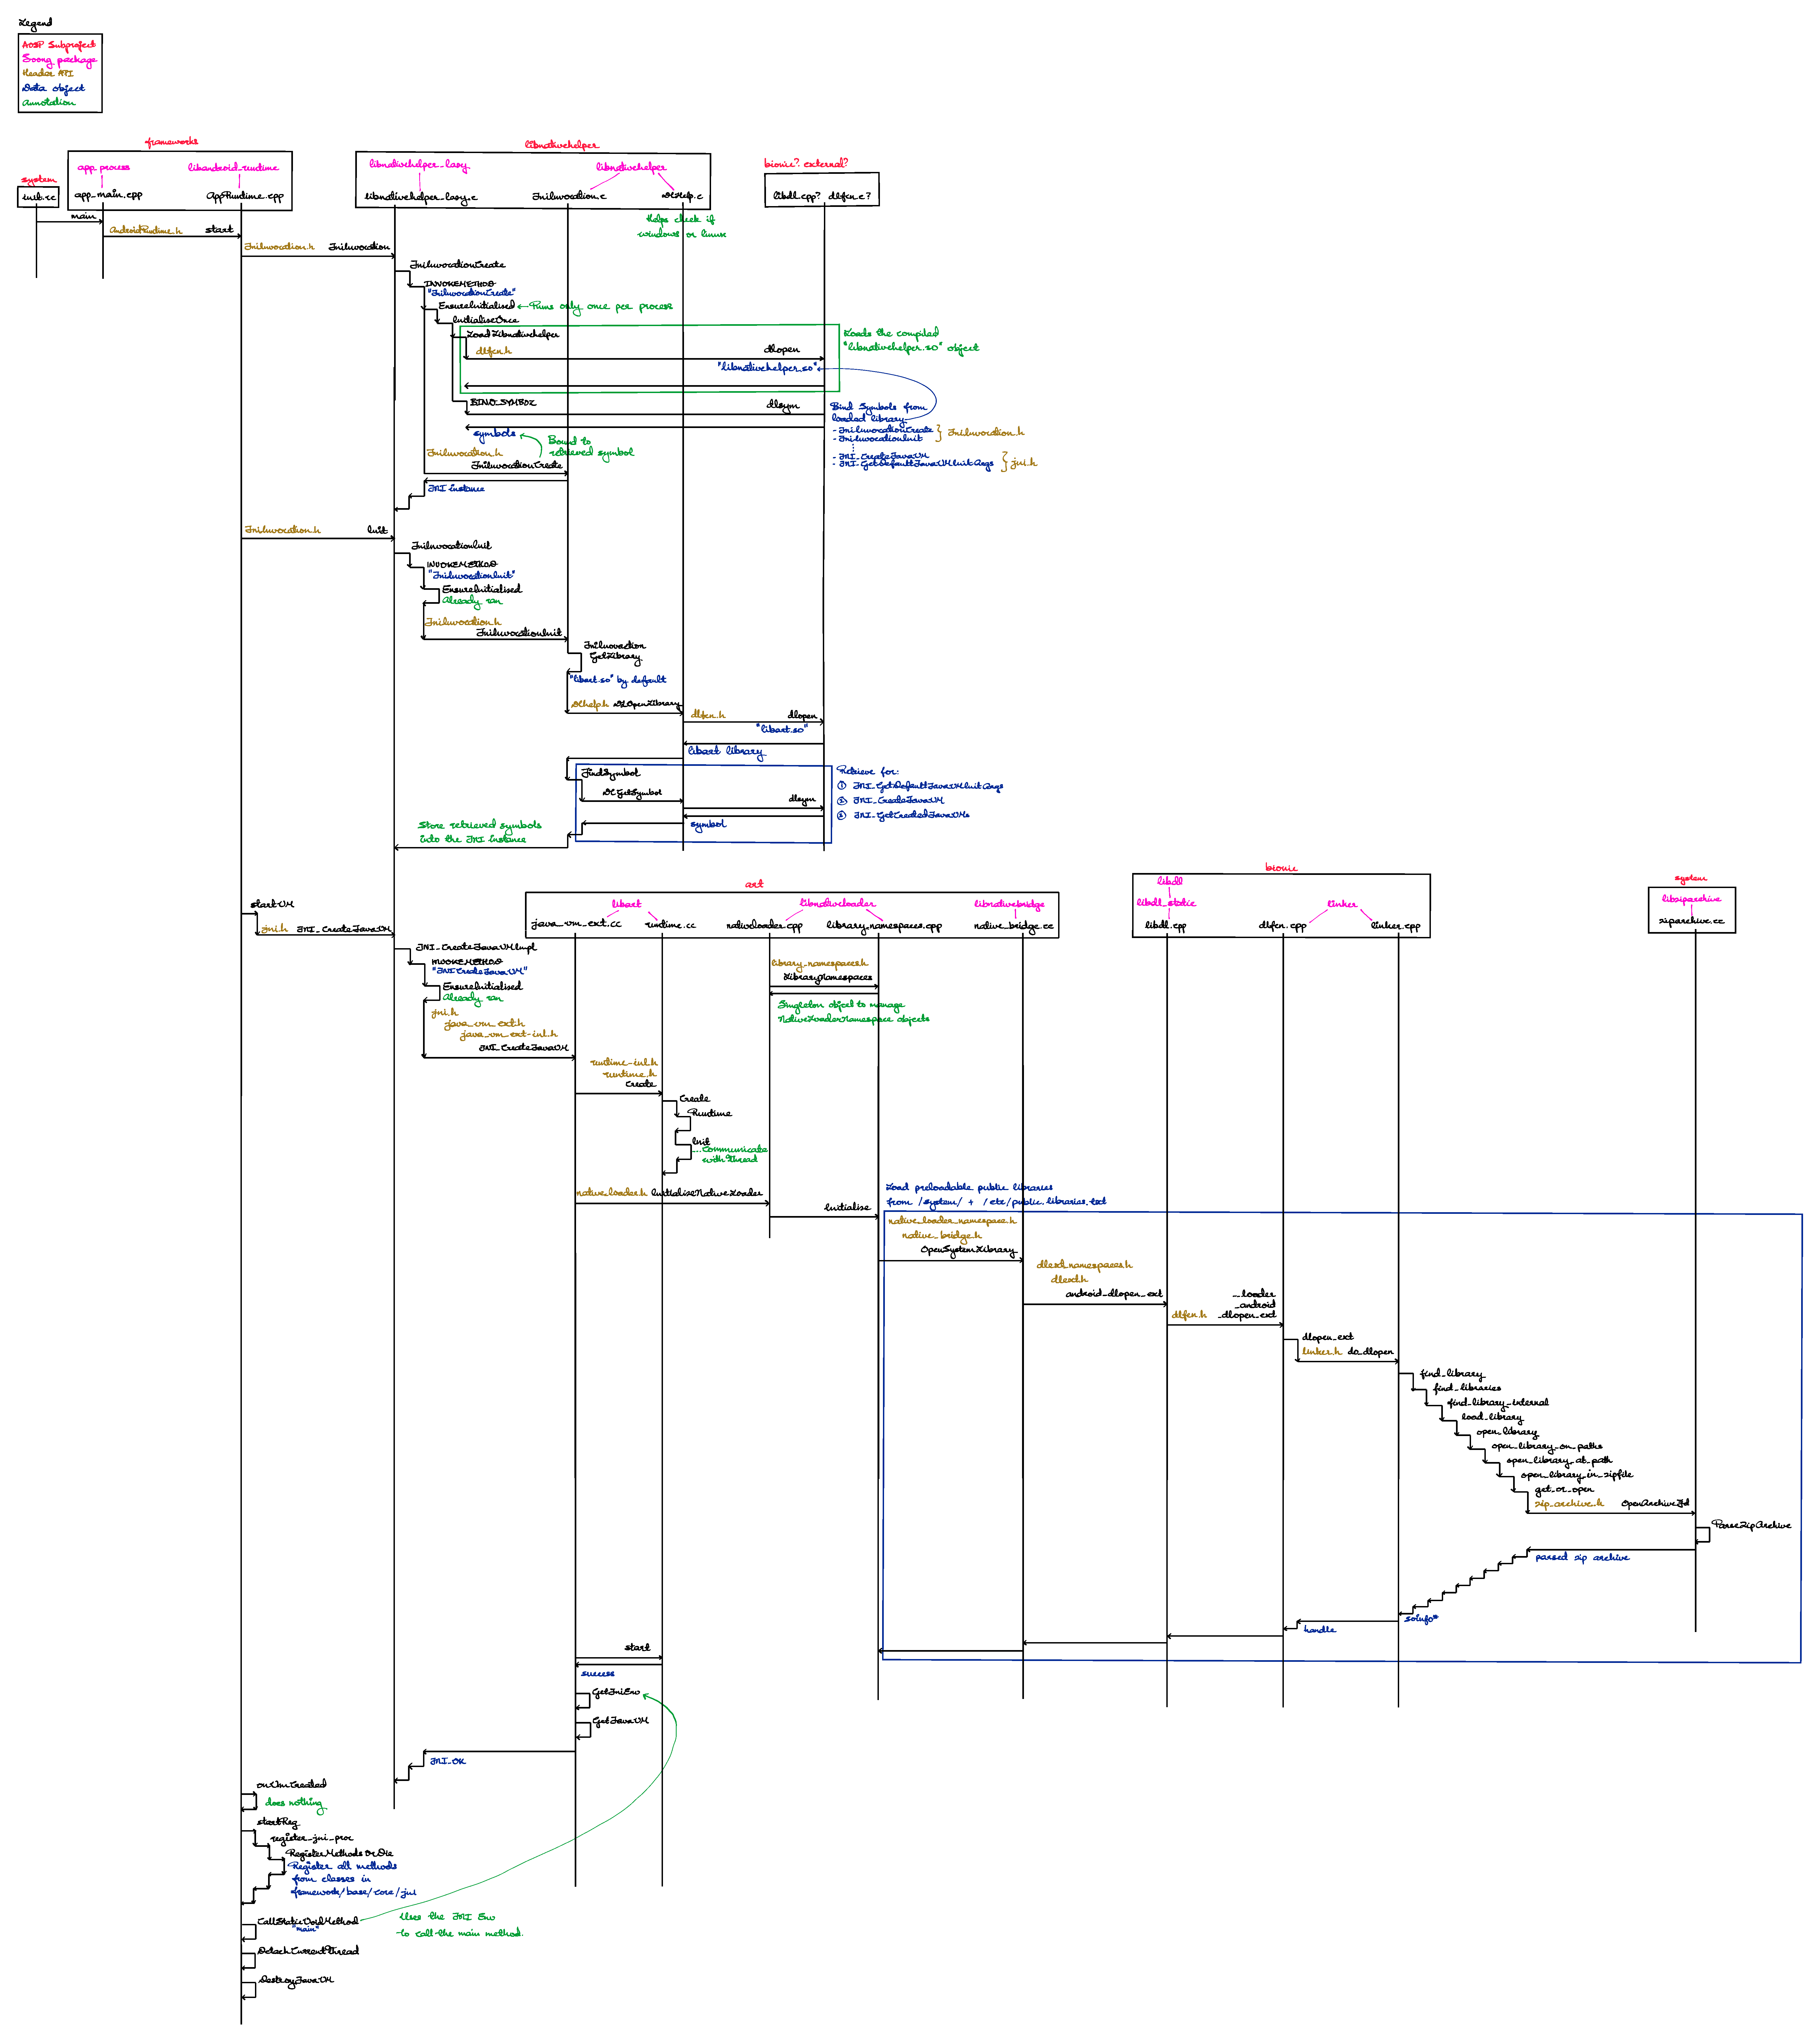
\includepdf[pages=-, scale=.95,pagecommand={}]{entries/2024/01/01/art.pdf}

% \begin{itemize}
% \item \textbf{Domain.} The context of the process that is acting upon something.
% \item \textbf{Type.} The context of the resource on which the process is acting.
% \item \textbf{Class.} The object class of the resource (e.g. \textit{file} or \textit{socket}).
% \item \textbf{Permissions.} The permissions that are allowed given the \textit{domain}, \textit{type} and \textit{class}.
% \end{itemize}

% SELinux rule syntax:


% \subsubsection{Decoding Permission Denial Message}

% Message:
% \begin{lstlisting}
% type=AVC msg=audit(1363289005.532:184): avc:  denied  { read } for  pid=29199 comm="Trace" 
% name="online" dev="sysfs" ino=30 scontext=staff_u:staff_r:googletalk_plugin_t 
% tcontext=system_u:object_r:sysfs_t tclass=file
% \end{lstlisting}

% \begin{longtable}{p{.15\linewidth}p{.15\linewidth}p{.65\linewidth}} 
% \toprule
% Log part & Name & Description \\
% \midrule
% \endhead

% \texttt{type=AVC}
% &Log type
% &Only in the \texttt{audit.log} file; it informs the user what kind of audit log type this is. 
% \\

% \midrule
% \caption{Permission Denied Syntax} 
% \label{tab:permissiondeniedsyntax}
% \end{longtable}


% \subsubsection{SELinux Architecture}

% SELinux consists of four main components: object managers (OM), access vector cache (AVC), security server, and security policy as show below:
% \begin{figure}[H]
%     \centering
%     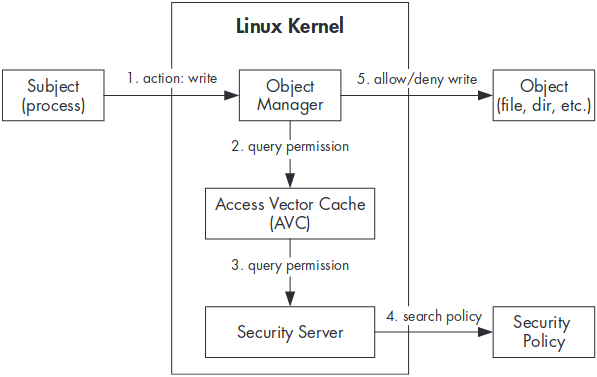
\includegraphics[width=.85\linewidth]{entries/2023/12/10/selinux.png}
%     \caption{SELinux Components}
%     \label{fig:selinux}
% \end{figure}
